\documentclass[a4paper,12pt]{article}

\usepackage{cmap}		
\usepackage[utf8]{inputenc}			
\usepackage[english,russian]{babel}
\usepackage{framed}
\usepackage{hyperref}
\usepackage{amsmath}
\usepackage{graphicx}
\usepackage[colorinlistoftodos]{todonotes}
\usepackage{wrapfig}
\usepackage{lipsum}
\usepackage{listings}
\usepackage{color}
\usepackage{indentfirst}
\usepackage{times}
\usepackage{textcomp}
\usepackage{smartdiagram}
\usepackage{caption}
\usesmartdiagramlibrary{additions}
\usepackage{tikz}
\usepackage{multicol}
\usepackage{lipsum}
\usepackage{mwe}
\usepackage{floatrow}
\usepackage{subfig}
\usepackage{algorithm}
\usepackage{algorithmic}
\usepackage[noend]{algpseudocode}
\usetikzlibrary{arrows,shapes}

\definecolor{mygray}{rgb}{0.4,0.4,0.4}
\definecolor{mygreen}{rgb}{0,0.8,0.6}
\definecolor{myorange}{rgb}{1.0,0.4,0}

\lstdefinestyle{customc}{
  belowcaptionskip=1\baselineskip,
  breaklines=true,
  frame=L,
  xleftmargin=\parindent,
  language=C,
  showstringspaces=false,
  basicstyle=\footnotesize\ttfamily,
  keywordstyle=\bfseries\color{green!40!black},
  commentstyle=\itshape\color{purple!40!black},
  identifierstyle=\color{blue},
  stringstyle=\color{orange},
  numbers=left,
  numbersep=12pt,
  numberstyle=\small\color{mygray},
}
\lstset{escapechar=@,style=customc}

\newcommand{\HRule}{\rule{\linewidth}{0.5mm}}
\DeclareMathOperator*{\argmax}{arg\,max}
\DeclareMathOperator*{\argmin}{arg\,min}

\begin{document}

\begin{titlepage}
\begin{center}

\textsc{\Large Московский Государственный Технический Университет имени Н.Э.Баумана}\\
\textsc{\large (Национальный Исследовательский Университет)}\\[1.5cm]

% Upper part of the page. The '~' is needed because \\
% only works if a paragraph has started.

\includegraphics[width=0.3\textwidth]{img/logo.png}~\\[1cm]

\textsc{\Large Научно-исследовательская работа}\\[0.5cm]

% Title
\HRule \\[0.4cm]
{ \LARGE \bfseries Методы обучения с подкреплением \\ для решения задач сборки \\[0.4cm] }

\HRule \\[1.5cm]

% Author and supervisor
\noindent
\begin{minipage}{0.4\textwidth}
\begin{flushleft} \large
\emph{Студент:}\\
Юнес \textsc{А.~Ю.}
\end{flushleft}
\end{minipage}%
\begin{minipage}{0.4\textwidth}
\begin{flushright} \large
\emph{Рукаводитель:} \\
Ющенко \textsc{А.~С.}
\end{flushright}
\end{minipage}

\vfill

% Bottom of the page
{\large \today}

\end{center}
\end{titlepage}

\newpage
\begin{abstract}
    The standard control methods in robotics are based on the dynamical model of the robot, and also on the model of the dynamics of the environment to build the needed closed loop control scheme; in the real world to realize such methods for manipulators, we have to follow the following steps: (1) taking an observation of the environment using cameras or sensors (2) estimating the state of the robot and the task (e.g,position of the end-effector and the goal position) (3) planing the trajectory of motion of the end-effector to achieve the task (4) using low-level controllers (or force controller for harder tasks) to ensure following the planned path by minimizing the errors (5) sending the resulting commands to the joints of the robot. The errors which are occurred in each step, accumulated to produce a cumulative error making the control process hard to realize with desired accuracy.\\ \par
    We suggest using the machine learning to achieve end-to-end mapping directly from observations to joints' motors commands, exploit the last deep learning revolution in using deep (large) neural networks. The state of the art deep reinforcement learning algorithms, that tried to handle robotic tasks can be classified to two major classes: (1) model-free algorithms: (like TRPO,PPO,DDPG) which can learn to achieve the task after sampling training sets from interacting with environment, so we can consider the robot's model as a black-box (2)model-based algorithms: depends on a known (or learned) transition model of the environment. The model-free algorithms need days of training to learn basic robotic tasks. On the other hand, model-based algorithms can learn much more faster (less than an hour), but can't adapt to unforeseen situation (the learned model is no longer valid).\\ \par
    We intend in that research to develop a data-efficient model-free algorithm, which can get the benefits of the both classes of deep reinforcement learning algorithms, and learn the assembly task (which is considered as a hard problem in standard robotic control) in a considerable small period of time.
\end{abstract}
\newpage
\tableofcontents

\newpage
\listoffigures
\listoftables
 
\newpage
\section{Введение}
\subsection{классическое управление робототехники}
Стандартные методы управления в робототехнике основаны на динамической модели робота, а также на модели динамики среды, которых нужны для построения необходимой схемы замкнутого контура управления; в реальном мире для реализации таких методов, мы должны следовать следующие шаги:
\begin{enumerate}
    \item Взятие наблюдения состояниея окружающей среды с помощью камер или датчиков
    \item Оценование состояния робота и задач (например, положение манипулятора схвата и положение цели) 
    \item Планирование траектории движения манипулятора схвата для достижения задач
    \item Использование низкоуровневых контроллеров (или контроллеров силы на более сложные задачи), чтобы обеспечить запланированная траектории за счет минимизации ошибок.
    \item Отправка полученных команд на стыки робота
\end{enumerate} 
\begin{center}
\captionof{figure}{классическое управление}
\smartdiagramset{
uniform color list=gray!60!blue!20 for all items,
text width=5cm,
back arrow disabled=true,
}
\smartdiagram[flow diagram:vertical]{наблюдение,оценка состояния,планирование движения,низкий уровень контроля,мотор команды}
\end{center}

\subsection{глубокое обучение робототехники}
Ошибки, которые произошли в каждом шаге классического управления робототехники, накопленное, и произвести совокупную ошибку, делая процесс контроля сложно реализовать с требуемой точностью, с другой стороны алгоритм управления поддержать только конкретную задачу. Это объясняет, почему такие алгоритьы не могут легко адаптироваться к новой задаче, и совсем не справляются с незнакомой. Но и решение этой проблемы было найдено, благодаря новым методам и алгоритмам обучения, которые позволяют роботам учиться гораздо быстрее и эффективнее.\par
Существуют различные методы, позволяющие роботу обучаться, а некоторые уже дают многообещающие результаты в исследовательских лабораториях по всему миру.\par
Один из подходов, в частности, имеет большое влияние в промышленной робототехнике. Глубокое обучение (deep learning), которое используется для обучения больших искусственных нейронных сетей. Некоторые компании стремятся использовать этот подход для обучения своих роботов.\par
Мы предлагаем использовать машинное обучение для достижения сквозного отображения непосредственно из наблюдений в команды двигателей суставов, использовать последнюю революцию глубокого обучения при использовании глубоких (больших) нейронных сетей.
\begin{center}
\captionof{figure}{глубокое обучение для управления робототов}
\smartdiagramset{
uniform color list=gray!60!blue!20 for all items,
text width=5cm,
back arrow disabled=true,
}
\smartdiagram[flow diagram:vertical]{наблюдение,Глубокая Нейронная Сеть,мотор команды}
\end{center}
\newpage

\subsection{Постановка задачи}

Промышленные роботы все больше и больше устанавливаются в различные индустрии для того чтобы решать сложных задач сборочного производства и высокой точности. Классический метод программирования научить роботу выполнять задачи промышленной сборки путем определения ключевых положений и движений используя блока управления. Этот способ программирования, как правило, утомительно и отнимает много времени. Даже после программировать, настройка параметров для развертывания робота на новой заводской линии занимает много времени из-за изменений среды.

Другой метод оффлайн программирование или моделирование. Этот метод может сократить время простоя реальных роботов, но в целом он может занять больше времени, чем онлайн-Программирование, включая время разработки моделирования и тестирования на роботе. Достаточно сложно представить реальный мир, включая вариации окружения со 100\% точностью в имитационной модели. Поэтому, этот автономный метод не достаточен для некоторых промышленных применений как подвергать механической обработке точности и гибкая погрузо-разгрузочная работа где необходимая точность выше чем точность робота.


\begin{figure}[h]%
    \centering
    \subfloat[]{{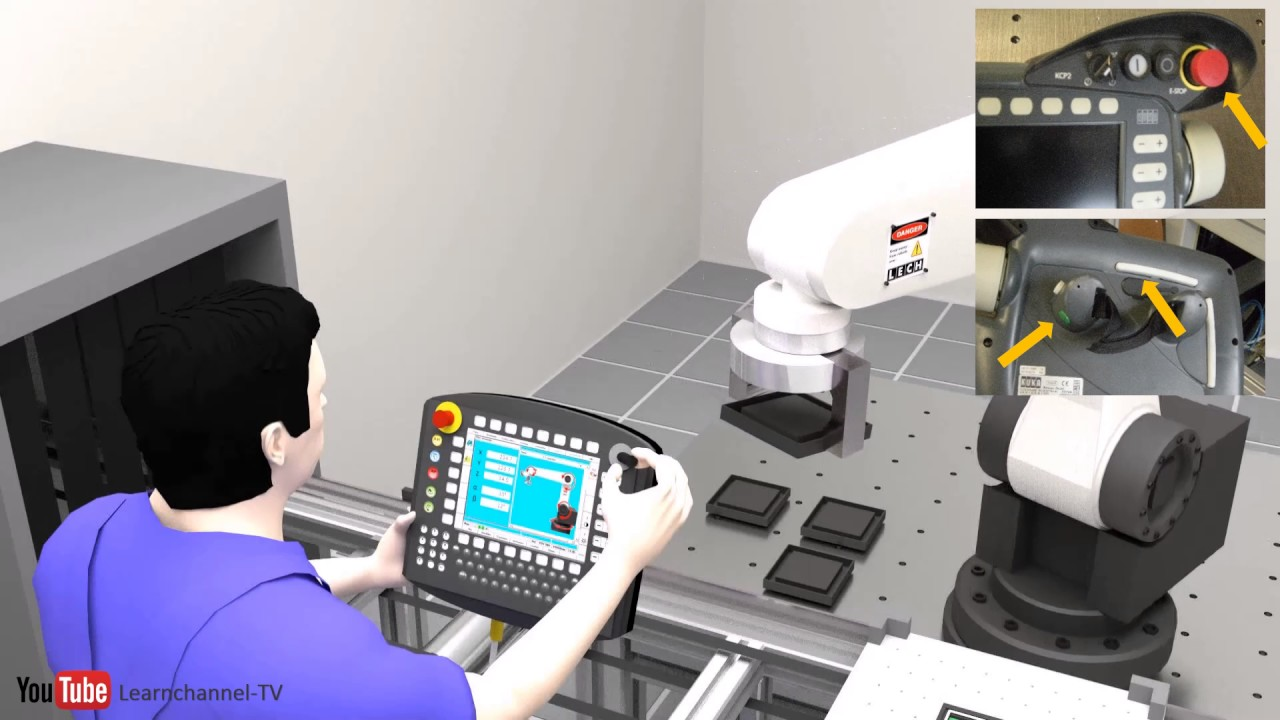
\includegraphics[width=5cm]{img/online.jpg} }}%
    \qquad
    \subfloat[]{{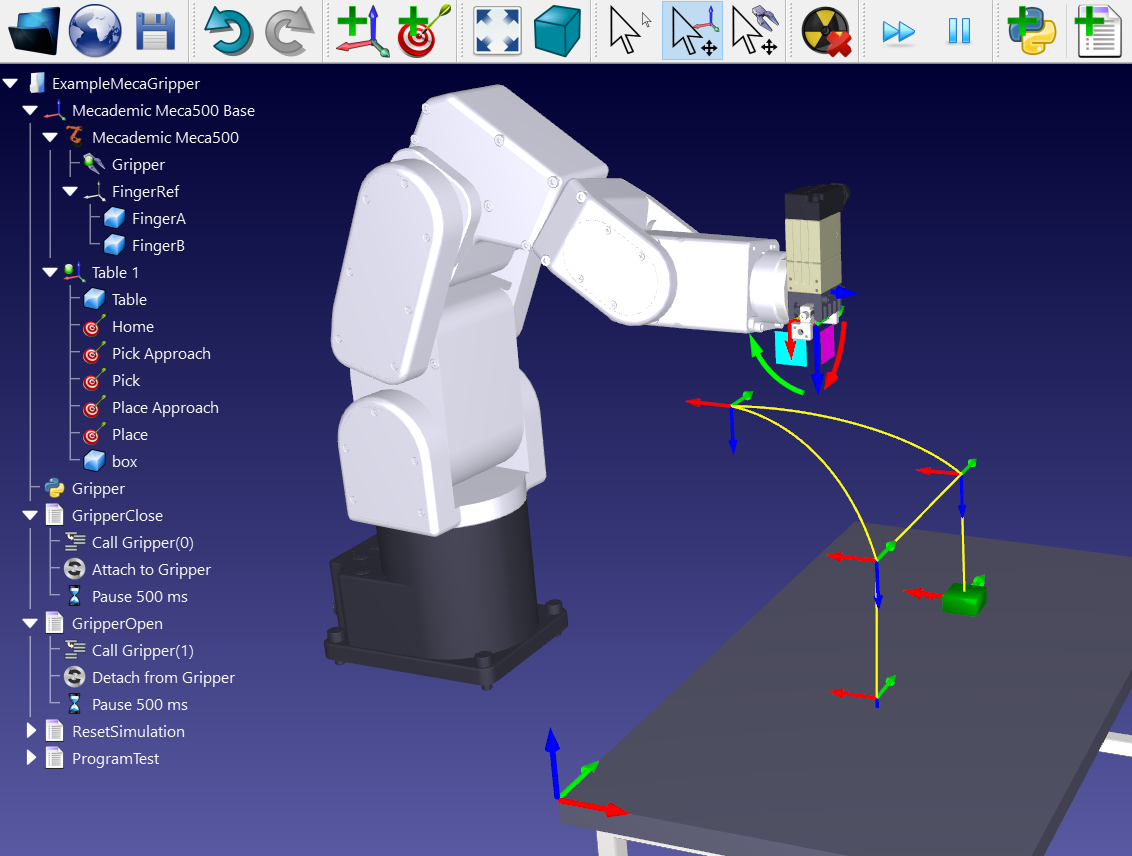
\includegraphics[width=5cm]{img/offline.png} }}%
    \caption{Онлайн (a) и Оффлайн (b) программирование}%
    \label{fig:example}%
\end{figure}

\newpage
В этой статье мы предлагаем подход к приобретению навыков, в котором низкая точность традиционных методов программирования компенсируется методом обучения без настройки параметров.
Для таких систем алгоритмы обучения с подкреплением (Reinforcement Learning) могут использоваться для того, чтобы робот мог изучать новые навыки методом проб и ошибок, используя процесс, который имитирует то, как люди учатся.

\begin{figure}[h]
    \centering
    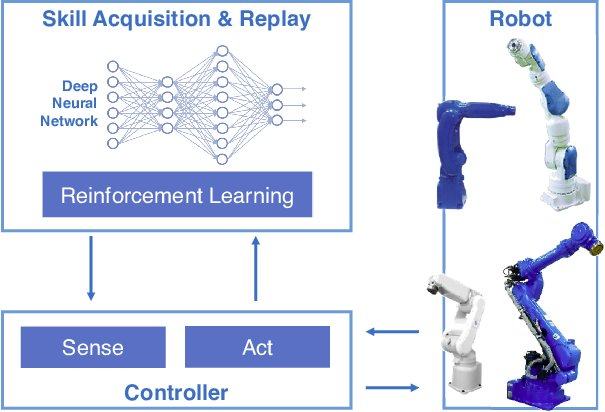
\includegraphics[width=6cm]{img/Rl-robot.jpg}
    \caption{структура системы обучения}
    \label{fig:my_label}
\end{figure}

Чтобы показать эффективность этого подхода, мы сосредоточимся на изучении задачи "плотный зазор цилиндрический стержня в отверстии" (Tight clearance cylindrical peg-in-hole task). Проблема отметки уровня для контролируемого сил робототехнического собрания. Точность, необходимая для выполнения этой задачи, превышает точность робота. В дополнение к плотному зазору отверстие можно опрокинуть в любом направлении, этом более добавочном к затруднению проблемы. Вместо использования сверхточных датчиков силы и момента мы полагаемся на камеру и датчики силы и положения, которыми оснащены большинство промышленных роботов.
\begin{figure}[h]%
    \centering
    \subfloat[]{{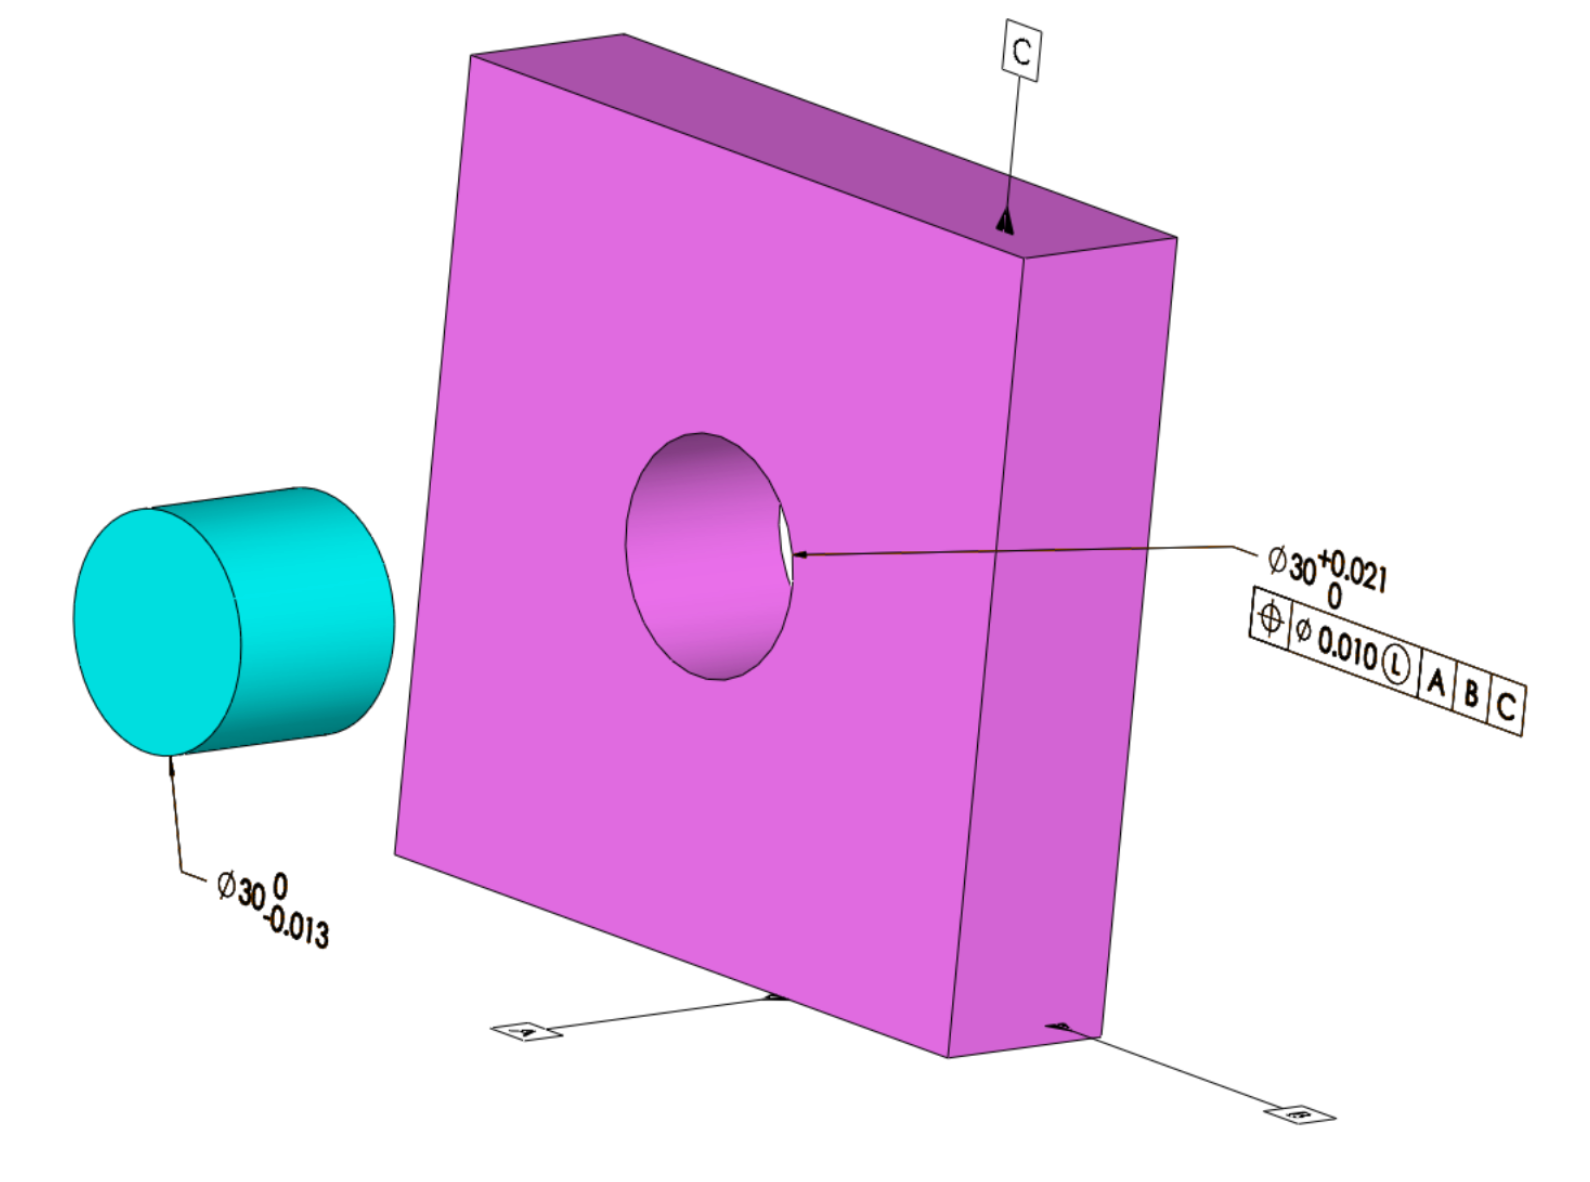
\includegraphics[width=5cm]{img/LMC.png} }}%
    \qquad
    \subfloat[]{{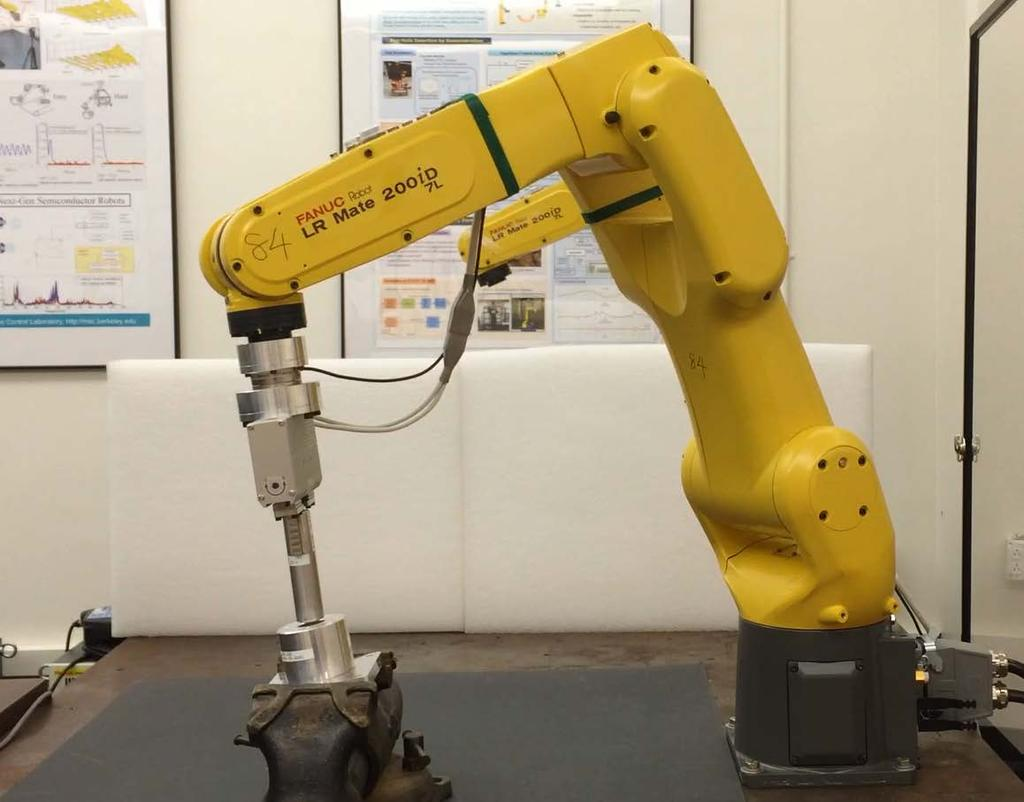
\includegraphics[width=5cm]{img/5-0.jpg} }}%
    \caption{плотный зазор цилиндрический стержня в отверстии}%
    \label{fig:example}%
\end{figure}

\newpage
\section{Направления исследований } 
\subsection{Обучения с подкреплением }
Обучение с подкреплением, идея которого была почерпнута в смежной области психологии, является подразделом машинного обучения, изучающим, как агент должен действовать в окружении, чтобы максимизировать некоторый долговременный выигрыш. Алгоритмы с частичным обучением пытаются найти стратегию, приписывающую состояниям окружающей среды действия, которые должен предпринять агент в этих состояниях. 
\begin{center}
\captionof{figure}{Обучения с подкреплением}
    \tikzstyle{block} = [rectangle, draw, 
    text width=8em, text centered, rounded corners, minimum height=4em]
    \tikzstyle{line} = [draw, -latex]
    \begin{tikzpicture}[node distance = 6em, auto, thick]
        \node [block] (Agent) {Агент};
        \node [block, below of=Agent] (Environment) {Окружение};
        \path [line] (Agent.0) --++ (4em,0em) |- node [near start,align=center]{Действие \\ $a_t$} (Environment.0);
        \path [line] (Environment.180) --++ (-4em,0em) |- node [near start,align=center] {Новая состояния \\ $s_{t+1}$ \\Награда (Выигрыш) \\$r_{t+1}$} (Agent.180);
    \end{tikzpicture}
\end{center}{}

Окружение обычно формулируется как марковский процесс принятия решений (МППР) с конечным множеством состояний, и в этом смысле алгоритмы обучения с подкреплением тесно связаны с динамическим программированием. Вероятности выигрышей и перехода состояний в МППР обычно являются величинами случайными, но стационарными в рамках задачи.
\begin{center}
\captionof{figure}{марковский процесс принятия решений}
 \begin{tikzpicture}[->, >=stealth', auto, thick, node distance=3cm]

    \tikzstyle{round}=[thick,draw=black,circle]

    \node[round] (s0) {$s_0$};
    \node[round,right= 25mm of s0] (s1) {$s_1$};
    \node[round,above right=7mm and 10mm of s0] (a1){$a_1$};
    \node[round,right= 25mm of s1] (s2) {$s_2$};
    \node[round,above right=7mm and 10mm of s1] (a2){$a_2$};
    \node[round,above right=7mm and 10mm of s2] (a3){$a_3$};

    \path (s0) edge node[below] {$p(s_{t+1}|s_t,a_t)$}(s1)
          (s0) edge node {$\pi_\theta$} (a1)
          (a1) edge node {} (s1);
    \path (s1) edge node[below] {$p(s_{t+1}|s_t,a_t)$}(s2)
          (s1) edge node {$\pi_\theta$} (a2)
          (a2) edge node {} (s2);
    \path (s2) edge node {$\pi_\theta$} (a3);
\end{tikzpicture}
\end{center}
$M={S,A,\tau,r}$\\
Состояния : $s \in S$ \\
Действия : $a \in A$ , $a \sim \pi(a_t|s_t)$ , $\sum_{a}\pi(a|s)=1$\\
Вероятность переходов : $p(s_{t+1}|s_t,a_t)\in \tau $ , $\sum_{s'}p(s'|s,a)=1$\\
Функция вознаграждения : $ r : S \times A \to R $ \\
Марковское свойства : $p(s_{t+1}|s_t,a_t,..,s1,s1)=p(s_{t+1}|s_t,a_t)$

При обучении с подкреплением, в отличии от обучения с учителем,не предоставляются верные пары „входные данные-ответ“, а принятие субоптимальнх решений (дающих локальный экстремум) не ограничивается явно. Обучение с подкреплением пытается найти компромисс между исследованием неизученных областей и применением имеющихся знаний. Баланс изучения-применения при обучении с подкреплением исследовался в задаче многорукого бандита.

Формально простейшая модель обучения с подкреплением состоит из:
\begin{itemize}
    \item Множества состояний окружения S;
    \item Множества действий A;
    \item Множества вещественнозначных скалярных „выигрышей“. 
\end{itemize}

В произвольный момент времени t агент характеризуется состоянием $s_t \in S$ и множеством возможных действий $A(s_t)$. Выбирая действие $a \in A(s_t)$, он переходит в состояние $s_{t+1}$ и получает выигрыш $r_t$. Основываясь на таком взаимодействии с окружающей средой, агент, обучающийся с подкреплением, должен выработать стратегию $\pi: S \to A$, которая максимизирует величину $R=r_0 + r_1+\cdots+r_n$ в случае МППР, имеющего терминальное состояние, или величину

        $$R=\sum_t \gamma^t r_t$$

для МППР без терминальных состояний (где $0 \leq \gamma \leq 1$ —- дисконтирующий множитель для „предстоящего выигрыша“).

Таким образом, обучение с подкреплением особенно хорошо подходит для решения задач, связанных с выбором между долгосрочной и краткосрочной выгодой. Оно успешно применялось в различных областях, таких как робототехника, управление лифтами, телекоммуникации,шашки и нарды. 
\newpage
\subsection{Алгоритмы обучения с подкреплением}
Теперь, когда была определена функция выигрыша, нужно определить алгоритм, который будет использоваться для нахождения стратегии, обеспечивающей наилучший результат.

Наивный подход к решению этой задачи подразумевает следующие шаги:
\begin{itemize}
    \item опробовать все возможные стратегии;
    \item выбрать стратегию с наибольшим ожидаемым выигрышем. 
\end{itemize}
    
Первая проблема такого подхода заключается в том, что количество доступных стратегий может быть очень велико или же бесконечно. Вторая проблема возникает, если выигрыши стохастические — чтобы точно оценить выигрыш от каждой стратегии потребуется многократно применить каждую из них. Этих проблем можно избежать, если допустить некоторую структуризацию и, возможно, позволить результатам, полученным от пробы одной стратегии, влиять на оценку для другой. Двумя основными подходами для реализации этих идей являются оценка функций полезности и прямая оптимизация стратегий.

Подход с использованием функции полезности использует множество оценок ожидаемого выигрыша только для одной стратегии $\pi$ (либо текущей, либо оптимальной). При этом пытаются оценить либо ожидаемый выигрыш, начиная с состояния s, при дальнейшем следовании стратегии $\pi$.Функция ценности состояния :

        $$V(s)=E[R|s,\pi]$$

либо ожидаемый выигрыш, при принятии решения a в состоянии s и дальнейшем соблюдении $\pi$. Функция цинности состояния-действия :

        $$Q(s,a)=E[R|s,\pi,a]$$

Если для выбора оптимальной стратегии используется функция полезности Q, то оптимальные действия всегда можно выбрать как действия, максимизирующие полезность. Если же мы пользуемся функцией V, необходимо либо иметь модель окружения в виде вероятностей P(s'|s,a), что позволяет построить функцию полезности вида

        $$Q(s,a)=\sum_{s'}V(s')P(s'|s,a)$$
\newpage
либо применить т.н. метод исполнитель-критик (Actor-Critic), в котором модель делится на две части:
\begin{enumerate}
    \item Критик (Critic), оценивающий полезность состояния V
    \item Исполнитель (Actor), выбирающий подходящее действие в каждом состоянии.
\end{enumerate}

\begin{figure}[h]
\captionof{figure}{Метод исполнитель-критик (Actor-Critic)}
    \centering
    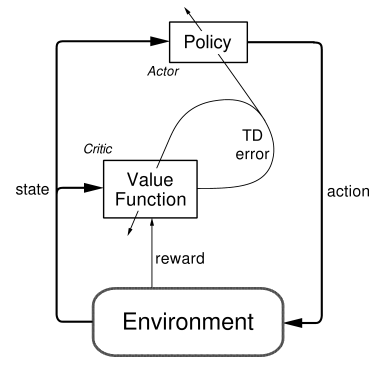
\includegraphics[width=6cm]{img/actor.png}
    \label{fig:actor-critic}
\end{figure}

Имея фиксированную стратегию $\pi$, оценить $E[R|\cdot]$ при $\gamma=0$ можно просто усреднив непосредственные выигрыши. Наиболее очевидный способ оценки при $\gamma>0$ — усреднить суммарный выигрыш после каждого состояния. Однако для этого требуется, чтобы МППР достиг терминального состояния (завершился).

Поэтому построение искомой оценки при $\gamma>0$ неочевидно. Однако, можно заметить, что R образуют рекурсивное уравнение Беллмана:

        $$E[R|s_t]=r_t+\gamma E[R|s_{t+1}]$$

Подставляя имеющиеся оценки, V, и применяя метод градиентного спуска с квадратичной функцией ошибок, мы приходим к алгоритму обучения с временными воздействиями.

В простейшем случае и состояния, и действия дискретны и можно придерживаться табличных оценок для каждого состояния. Другие похожие методы: Адаптивный эвристический критик (Adaptive Heuristic Critic, AHC), SARSA и Q-обучение (Q-learning). Все вышеупомянутые используют различные методы приближения, но в некоторых случаях сходимость не гарантируется. Для уточнения оценок используется метод градиентного спуска или метод наименьших квадратов в случае линейных приближений.

Указанные методы не только сходятся к корректной оценке для фиксированной стратегии, но и могут быть использованы для нахождения оптимальной стратегии Для этого в большинстве случаев принимают стратегию с максимальной оценкой, принимая иногда случайные шаги для исследования пространства. При выполнении некоторых дополнительных условий существуют доказательства сходимости упомянутых методов к оптимальной стратегии. Однако, эти доказательства гарантируют только асимптотическую сходимость, в то время как поведение алгоритмов обучения с подкреплением в задачах с малыми выборками мало изучено, не считая некоторых очень ограниченных случаев.

Альтернативный метод поиска оптимальной стратегии — искать непосредственно в пространстве стратегий. Таки методы определяют стратегию как параметрическую функцию $\pi (s,\theta )$ с параметром $\theta$. Для настройки параметров применяются градиентные методы. Однако, применение градиентных методов осложняется тем, что отсутствует информация о градиенте. Более того, градиент тоже приходится оценивать через зашумлённые результаты выигрышей. Так как это существенно увеличивает вычислительные затраты, может быть выгоднее использовать более мощные градиентные методы, такие как метод скорейшего спуска. Алгоритмы, работающие напрямую с пространством стратегий привлекли значительное внимание в последние 5 лет и в данный момент достигли достаточно зрелой стадии, но до сих пор остаются активным полем для исследований. Существуют и другие подходы, такие как метод отжига, применяемые для исследования пространства стратегий. 
\\

Самые важные современие адгоритмы обучения с подкреплением:
\begin{enumerate}
    \item Алгоритмы с непрерывными моделями: DQN (2013), DDPG (2015)
    \item Алгоритмы градиента стратегии: TRPO (2015), PPO (2017)
\end{enumerate}
\newpage
\subsection{Глубокий детерминированный градиент политики}
(Deep Deterministic Policy Gradient DDPG):
\subsubsection{Основные шаги выполнения алгоритма:}
\begin{enumerate}
    \item Выираем действие $a_t$, система переходить в новое состояние, определяя $(s_t,a_t,r_t,s_{t+1})$
    \item Вычисляем цель согласно $y_i=r_i+\lambda Q_\theta(s_{t+1},\mu_\phi(s_{t+1}))$
    \item Обновляем параметры функции ценности (критика):
    $$\theta \leftarrow \theta - \alpha \frac{\delta Q_\theta(s_t,a_t)}{\delta\theta} (Q_\theta(s_t,a_t)-y_t)$$
    \item Обновляем параметры функции действия (актор- исполнитель):
    $$\phi \leftarrow \phi-\Beta \frac{\delta Q_\theta (s_t,a_t)}{\delta \mu_\phi}\frac{\delt a \mu_\phi (s_t)}{\delta \phi}$$
\end{enumerate}

\subsubsection{Обзор алгоритма:}
В этом алгоритме возникает проблема отсутствия гарантий сходимости; в отличии от конечных моделей, стратегия может быть улучшена локально, так как изменеие параметра $\alpha$ влечет изменеие ценности $Q$ во многих состоянях. Оценка $Q$ становится смещенной, неизвестно к чему она сходится ли вообще.

Это проблема будить важно в более сложных задачах с большей размерностью, более отсроченным вознаграждением, более сложной стратегией. Когда важна близость к оптимальному решению.

\newpage
\subsection{Градиент стратегии}
(Policy gradient):
Если у нас $\pi(a_t|s_t)$ - стратегия испольнителя (актора), $p(s_{t+1}|s_t,a_t)$ - вероятность перехода, и $\tau=\{s_0,a_0,s_1,a_1\}$ - траектория; тогда распределение трактория:
\begin{align*}
    p_\theta(\tau)&=p(s_0)\pi(a_0|s_0)p(s_1|s_0,a_0)\pi(a_1|s_1)p(s_2|s_1,a_1)...=\\
    &= p(s_0)\prod_{t=0}^{N}\pi(a_t|s_t)p(s_{t+1}|s_t,a_t)
\end{align*}
Цель оптимизация - максимизация ожидания совокупного вознаграждения:
$$J(\theta)=\max_{\theta} E_{\tau\sim p_\theta}[r(\tau)]$$
где : $$r(\tau)=\sum_{t=0}^{N}r(s_t,a_t)$$
Градиент целевой функции:
\begin{align*}
    \nabla E_{x\sim p_\theta} [F(x)]&=\nabla_\theta \sum_{x} p_\theta (x) f(x)=\\
    &=\sum_x p_\theta(x)\nabla_\theta \ln{p_\theta(x)f(x)}=\\
    &=E_{x\sim p_\theta}[\nabla_\theta \ln{p_\theta (x) f(x)}]\\
    \nabla_\theta \ln{p_\theta(\tau)}&=\nabla_\theta (\ln{p(s_0)+\sum_t (\ln{\pi_\theta (a_t|s_t)}+\ln{p(s_{t+1}|s_t,a_t)})})=\\
    &=\sum_t \nabla_\theta \ln{\pi_\theta (a_t|s_t)}
\end{align*}

$$\nabla_\theta J(\theta)=E_{\tau \sim p_\theta}[\,\sum_{t=0}^{N}\nabla \ln{\pi_\theta(a_t|s_t)r(\tau)}]\,$$
Недостатки градиента стратегии:
\begin{enumerate}
    \item Большая дисперсия:\\
    Уменьшение дисперсии путем использования базового члена зависящий от состояния  
    \item Репараметризационная неинвариантность:\\
    Ведущая к медленной сходимости. Решена в следуюших алгоритмах.
\end{enumerate}
\subsubsection{Натуральный градиент стратегии}
(Natural Policy Gradient NPG):
Нам нужно оптимизировать цель, причем новая стратегия $\pi_\theta $ и старая стратегия $ \pi_{\theta_{old}}$ близки друг к другу, поэтому задача оптимизации может быть сформирована как:
$$\theta \leftarrow \argmax_{\theta '} \sum_{t} E_{s_t\sim \p_\theta (s_t)} [\, E_{a_t\sim \pi_\theta (a_t|s_t)}[\,\frac{\pi_{\theta '}(a_t|s_t)}{\pi_\theta (a_t|s_t)} \gamma^t A^{\pi_\theta}(s_t,a_t)]\,]\,$$
$$s.t. D_{KL}(\pi_{\theta '}(a_t|s_t)||\pi_\theta(a_t|s_t))\leq \epsilon$$
где $A(s_t,a_t)=Q(s_t,a_t)-V(s_t)$ функция преимущества (advantage function)\\
используя приближение Тейлора первого порядка для целевой функции:
$$\theta ' \leftarrow \nabla_\theta J(\theta)^T (\theta ' - \theta)$$
и используя приближение Тейлора второго порядка для ограничения:
$$D_{KL}(\pi_{\theta '}||\pt_\theta)\approx \frac{1}{2}(\theta -\theta ')^T F(\theta - \theta ')$$
Тнформация Фишера $F=\frac{\delta^2 D_{KL}(\theta||\theta ')}{\delta\theta\delta\theta '}|_{\theta '=\theta}$\\

Восстановливанием репараметризационную инвариантность:
$$\theta ' \leftarrow \theta+\alpha F^{-1}\nabla_\theta J(\theta)$$

Натуральный градиент: подъем градиента в вероятностном пространстве, а не в пространстве параметров

\newpage
\subsubsection{Оптимизация политики доверительного региона}
(Trust Region Policy Optimization TRPO):
\begin{algorithm}[H]
    \caption{Trust Region Policy Optimization}
    \label{alg1}
\begin{algorithmic}[1]
    \STATE Input: initial policy parameters $\theta_0$, initial value function parameters $\phi_0$
    \STATE Hyperparameters: KL-divergence limit $\delta$, backtracking coefficient $\alpha$, maximum number of backtracking steps $K$
    \FOR{$k = 0,1,2,...$}
    \STATE Collect set of trajectories ${\mathcal D}_k = \{\tau_i\}$ by running policy $\pi_k = \pi(\theta_k)$ in the environment.
    \STATE Compute rewards-to-go $\hat{R}_t$.
    \STATE Compute advantage estimates, $\hat{A}_t$ (using any method of advantage estimation) based on the current value function $V_{\phi_k}$.
    \STATE Estimate policy gradient as
        \begin{equation*}
        \hat{g}_k = \frac{1}{|{\mathcal D}_k|} \sum_{\tau \in {\mathcal D}_k} \sum_{t=0}^T \left. \nabla_{\theta} \log\pi_{\theta}(a_t|s_t)\right|_{\theta_k} \hat{A}_t.
        \end{equation*}
    \STATE Use the conjugate gradient algorithm to compute
        \begin{equation*}
        \hat{x}_k \approx \hat{H}_k^{-1} \hat{g}_k,
        \end{equation*}
        where $\hat{H}_k$ is the Hessian of the sample average KL-divergence.
    \STATE Update the policy by backtracking line search with
        \begin{equation*}
        \theta_{k+1} = \theta_k + \alpha^j \sqrt{ \frac{2\delta}{\hat{x}_k^T \hat{H}_k \hat{x}_k}} \hat{x}_k,
        \end{equation*}
        where $j \in \{0, 1, 2, ... K\}$ is the smallest value which improves the sample loss and satisfies the sample KL-divergence constraint.
    \STATE Fit value function by regression on mean-squared error:
        \begin{equation*}
        \phi_{k+1} = \arg \min_{\phi} \frac{1}{|{\mathcal D}_k| T} \sum_{\tau \in {\mathcal D}_k} \sum_{t=0}^T\left( V_{\phi} (s_t) - \hat{R}_t \right)^2,
        \end{equation*}
        typically via some gradient descent algorithm.
    \ENDFOR
\end{algorithmic}
\end{algorithm}

\section{Заключение}
\subsection{}
\newpage
\begin{thebibliography}{9}
    \addcontentsline{toc}{section}{\refname}
    \bibitem{TRPO}   J. Schulman, S. Levine, P. Moritz, M. I. Jordan, and P. Abbeel. “Trust region policy optimization”. In:CoRR, abs/1502.05477 (2015).
    \bibitem{openai_gym} G. Brockman, V. Cheung, L. Pettersson, J. Schneider, J. Schulman, J. Tang, and W. Zaremba. “OpenAI Gym”. In: arXiv preprint arXiv:1606.01540 (2016).
    \bibitem{Sutton} Richard S Sutton and Andrew G Barto. Reinforcementlearning: An introduction, volume 1. MIT press Cambridge, 1998.
    \bibitem {task} Зенкевич С. Л., Ющенко А. С. Основы управления манипуляционными роботамиб Изд-во МГТУ им. Н. Э. Баумана, 2004
    \bibitem{survey} Deisenroth M.P., Neumann G., Peters J. A survey on policy search for robotics Found. Trends Robot., 2 (1–2) (2013), pp. 1-142
    \bibitem{data-efficient} Konstantinos Chatzilygeroudis, Roberto Rama, Rituraj Kaushik, Dorian Goepp, Vassilis Vassiliades, et al.. Black-Box Data-efficient Policy Search for Robotics. IEEE/RSJ International Conference on Intelligent Robots and Systems (IROS), Sep 2017, Vancouver, Canada

\end{thebibliography}

\end{document}

\usepackage[english,russian]{babel}